\documentclass[12pt,a4paper]{article}
\usepackage{ra_preamble}
\usepackage{longtable}
\usepackage{booktabs}

\title{\textbf{The Discreteness Constant:\\
Fine Structure Constant, Strong Coupling,\\and the Standard Model Spectrum\\
from Four-Dimensional Causal Geometry}\\[0.6em]
\large\normalfont Relational Actualism --- Paper~I}
\author{Joshua F.~Sandeman\\[0.4em]
\small Independent Researcher, Salem, Oregon\\
\small \texttt{sansuikyo@gmail.com} $\cdot$ \texttt{relationalactualism.org}}
\date{April 2026}

\begin{document}
\maketitle

\begin{abstract}
We derive the fine structure constant $\alpha_{\rm EM}^{-1}=137$ (exact integer, Lean~4 verified by \texttt{norm\_num} in RA\_D1\_Proofs.lean \statusLV), the strong coupling constant $\alpha_s(m_Z)=1/\sqrt{72}=0.11785$ (PDG: $0.1180\pm0.0009$, $0.13\%$ agreement, computation-verified \statusCV), and the complete Standard Model particle spectrum (five topology classes, 124 extensions, Lean~4 verified \statusLV) from the integers $(1,-1,9,-16,8)$ characterising the Benincasa--Dowker--Glaser (BDG) causal set action in four spacetime dimensions.  These integers are not free parameters: they are the unique solution to the requirement that the BDG discrete operator converges to the d'Alembertian $\Box$ in the Lorentzian continuum limit in $d=4$, a result established by Dowker and Glaser \cite{Dowker2013} independently of any physical measurement.

We prove that $d=4$ is the unique dimension satisfying two independent constraints: (C1)~the BDG Closure Theorem, establishing that exactly five topologically stable classes exist in $d=4$ corresponding to all five Standard Model particle types with no additional classes possible; and (C2)~the D4U02 selectivity condition, that the acceptance probability $P_{\rm acc}(\mu)$ has its first local maximum near the Planck density, proved here analytically for the first time by conditioning on $K=9N_2-16N_3+8N_4$ and applying modular arithmetic ($9\equiv1\pmod8$) to establish $P(S=1)>P(S=0)$ by a 3100:1 margin \statusDR.  The modular barrier is specific to $d=4$; it fails in all other dimensions.

Additional results from the same five integers, all without free parameters: the Koide lepton mass formula $K=2/3$ (first derivation from first principles, Lean~4 verified \statusLV); QCD confinement depths $L_g=3$, $L_q=4$ (Lean~4 verified \statusLV); proton mass $m_p=\sqrt{c_4}\Lambda_{\rm QCD}$ to $0.08\%$ \statusCV; cosmological baryon-to-dark ratio $f_0=5.42$ (Planck: $5.416$, $0.07\%$) \statusCV; the Roper resonance gap $290\,{\rm MeV}$ identified as a Kind~2 virtual process \statusCV; charge quantisation in units of $e/3$ from $N_2$ winding numbers; exact baryon number conservation; and $\theta_{\rm QCD}=0$ from DAG acyclicity.  A self-referential fixed point $\mu_{\rm fp}\approx\Delta S^*=0.60069$ and the D4U02 selectivity maximum together constitute a double restoring force that anchors the universe to the Planck operating point without fine-tuning.
\end{abstract}

\tableofcontents\bigskip

%═══════════════════════════════════════════════════════════════════════════════
\section{Introduction: Why the Coupling Constants Are a Mystery}\label{sec:intro}
%═══════════════════════════════════════════════════════════════════════════════

\subsection{The Standard Model's Unanswered Question}

The Standard Model of particle physics is one of the greatest intellectual achievements in the history of science.  It describes three of the four fundamental forces, classifies all known elementary particles, and makes quantitative predictions that have been confirmed to extraordinary precision.  The anomalous magnetic moment of the electron is predicted and measured to eleven decimal places --- a level of agreement unprecedented in physics.  The $W$ and $Z$ boson masses were predicted before their discovery.  The Higgs boson, predicted in 1964, was discovered forty-eight years later at exactly the predicted mass.

Yet for all its power, the Standard Model is profoundly incomplete as an explanation of nature.  It contains approximately twenty free parameters that must be determined by measurement rather than derived from first principles.  The most prominent of these is the dimensionless fine structure constant:
\begin{equation}
  \alpha_{\rm EM} = \frac{e^2}{4\pi\varepsilon_0\hbar c} \approx \frac{1}{137.036}
  \label{eq:alpha_def}
\end{equation}
This number governs the strength of all electromagnetic interactions.  The force between two electrons, the emission spectrum of hydrogen, the transparency of glass, the operation of every radio and optical device --- all depend on $\alpha_{\rm EM}$.  Yet the Standard Model takes this number as an input.  It cannot say why $\alpha_{\rm EM}^{-1}\approx137$ rather than $100$ or $200$.

The same is true of the strong coupling constant $\alpha_s$.  In quantum chromodynamics (QCD), the coupling ``runs'' with energy scale according to the renormalisation group.  Its measured value at the $Z$ boson mass scale is $\alpha_s(m_Z)=0.1180\pm0.0009$ \cite{PDG2024}.  The renormalisation group can evolve this value to other scales once the initial value is known, but the initial value itself is an empirical input.

Richard Feynman described the fine structure constant's inexplicability with characteristic directness: ``It's one of the greatest damn mysteries of physics: a magic number that comes to us with no understanding by man.  You might say the `hand of God' wrote that number, and we don't know how He pushed His pencil.  We know what kind of a dance to do experimentally to measure this number very accurately, but we don't know what kind of a dance to do on the computer to make this number come out --- without putting it in secretly!'' \cite{Feynman1985}.

Relational Actualism ends this mystery.  The coupling constants are not inputs.  They are outputs --- fixed-point eigenvalues of a four-dimensional causal geometry, fully determined by the requirement that a certain discrete operator converge to the wave operator in the continuum limit.

\subsection{Historical Attempts and Their Failures}

Before presenting the RA derivation, it is instructive to survey the history of attempts to explain $\alpha_{\rm EM}^{-1}=137$, because the failures of these attempts illuminate what a successful derivation must look like.

\paragraph{Eddington's numerology (1929--1946).}  Arthur Eddington derived $\alpha_{\rm EM}^{-1}=136$ from a counting argument about the number of independent degrees of freedom in a $16\times16$ antisymmetric matrix representing a proton-electron system \cite{Eddington1929}.  When measurements showed the value was closer to $137$, he revised his argument to obtain $137$.  This is the archetype of numerology: the expression is \emph{found} after the experimental value is known, not derived from independent principles.

\paragraph{Expressions involving $\pi$ and other constants.}  Many authors have noted that $\frac{1}{4}\sqrt[3]{\pi} + \pi^5\approx137$ or that various combinations of small integers produce $137$.  These are coincidences of arithmetic, not physics.

\paragraph{Anthropic arguments.}  The observation that stars burn stably only for a narrow range of $\alpha_{\rm EM}$ \cite{Barrow1988} explains why observers find themselves in a universe with the observed value, but only if many universes exist with different values --- a framework with its own severe problems.

\paragraph{Grand unified theories.}  In GUT scenarios, $\alpha_{\rm EM}$ and $\alpha_s$ unify at a high energy scale.  But the GUT coupling at unification is itself a free parameter, merely shifted to a new scale.

None of these approaches derives the coupling constants from independently established principles.  The RA derivation does.

\subsection{The Structural Distinction Between Derivation and Numerology}\label{sec:notnumerology}

The claim that $\alpha_{\rm EM}^{-1}=137$ follows from the arithmetic $144-7=137$ will immediately suggest numerology to a careful reader.  The distinction between derivation and numerology is real and structural, and it is essential to state it explicitly before any calculation appears.

\textbf{Numerology} has the following structure:
\begin{enumerate}
  \item The experimental value is known: $\alpha_{\rm EM}^{-1}=137.036$.
  \item A search is conducted through mathematical expressions until one produces this value.
  \item The expression is declared to be the ``true'' formula.
\end{enumerate}
The key defect of numerology is that the expression is \emph{chosen} for its output.  There is no independent reason, derivable without knowing the experimental value, why that particular expression should equal the coupling constant.

\textbf{The RA derivation} has the opposite structure:
\begin{enumerate}
  \item An independent geometric requirement is stated: the BDG discrete operator must converge to the d'Alembertian $\Box$ in four-dimensional Lorentzian spacetime.
  \item This requirement uniquely fixes the integers $(1,-1,9,-16,8)$.  This determination was made by Dowker and Glaser \cite{Dowker2013} without any reference to coupling constants.
  \item From these integers, the electromagnetic coupling emerges as a depth-ratio fixed point, and the strong coupling as a path-weight eigenvalue.
  \item The results are compared with experiment.
\end{enumerate}
The crucial test: if the experimental value of $\alpha_{\rm EM}^{-1}$ turned out to be $150$ instead of $137$, the BDG integers would still be $(1,-1,9,-16,8)$ --- they are determined by the d'Alembertian convergence requirement, not by the coupling constant.  The agreement between the BDG-derived value and the measured value is therefore a genuine prediction.  It could have been falsified.

A second test of non-numerology: the same five integers also derive the Koide lepton formula, QCD confinement depths, the proton mass, the baryon fraction, and the complete Standard Model particle spectrum.  A single five-integer input producing twelve independent results cannot be numerology.

\subsection{Overview of Results}

The complete list of results derived from the integers $(1,-1,9,-16,8)$ in this paper:

\begin{table}[ht]
\centering
\caption{All results derived from the five BDG integers, with no free parameters.  Status codes defined in Paper~V \cite{RA_P5}.}
\label{tab:overview}
\begin{tabular}{llp{4cm}p{2.5cm}l}
\toprule
ID & Quantity & RA Value & Exp.\ Value & Status \\
\midrule
L08 & $\alpha_{\rm EM}^{-1}$ & $137$; Wyler: $137.036$ & $137.036$ & \statusLV \\
L09 & Koide $K$ & $2/3$ & $0.6667$ & \statusLV \\
L10 & $L_g$, $L_q$ & $3$, $4$ & (confinement) & \statusLV \\
L11 & SM types & $5$ classes, $124$ ext. & 5 families & \statusLV \\
C01 & $\alpha_s(m_Z)$ & $1/\sqrt{72}=0.11785$ & $0.1180$ & \statusCV \\
C03 & $\Delta S^*$ & $0.60069$ nats & --- & \statusCV \\
C04 & $t^*$ & $0.274/g$ & --- & \statusCV \\
C06 & $m_p$ & $\sqrt{8}\,\Lambda_{\rm QCD}$ & $938.3$ MeV & \statusCV \\
C07 & Roper gap & $290$ MeV (Kind~2) & $290$ MeV & \statusCV \\
C08 & $f_0$ & $5.42$ & $5.416$ & \statusCV \\
D4U02a & $\mu^*>1$ & $P(S{=}1){>}P(S{=}0)$, 3100:1 & $\mu^*\approx1.019$ & \statusDR \\
D4U02u & $d=4$ unique & Modular barrier fails $d\ne4$ & --- & \statusDR \\
--- & $\theta_{\rm QCD}=0$ & DAG acyclicity & $<10^{-10}$ & \statusDR \\
--- & No $p$ decay & Baryon LLC topological & $>10^{34}$ yr & \statusDR \\
--- & 3 generations & Three BDG depth levels & 3 known & \statusDR \\
\bottomrule
\end{tabular}
\end{table}

\subsection{Organisation of This Paper}

Section~\ref{sec:bdg} derives the BDG action from first principles and establishes the uniqueness of the integers $(1,-1,9,-16,8)$.  Section~\ref{sec:dynamics} presents the Poisson-CSG actualization dynamics and establishes the threshold $\Delta S^*$.  Section~\ref{sec:uniqueness} proves $d=4$ uniqueness via both the SM Closure theorem (C1) and the D4U02 selectivity condition (C2), including the new analytic proof.  Section~\ref{sec:alphaEM} derives $\alpha_{\rm EM}^{-1}=137$.  Section~\ref{sec:alphas} derives $\alpha_s$ and its RG fixed points.  Section~\ref{sec:SM} presents the full Standard Model spectrum.  Section~\ref{sec:further} covers additional hadron and cosmological results.  Section~\ref{sec:fixed_point} establishes the self-referential fixed point.  Section~\ref{sec:predictions} catalogues falsifiable predictions.  Section~\ref{sec:discussion} discusses open problems and comparisons with previous work.

\begin{figure}[ht]
  \centering
  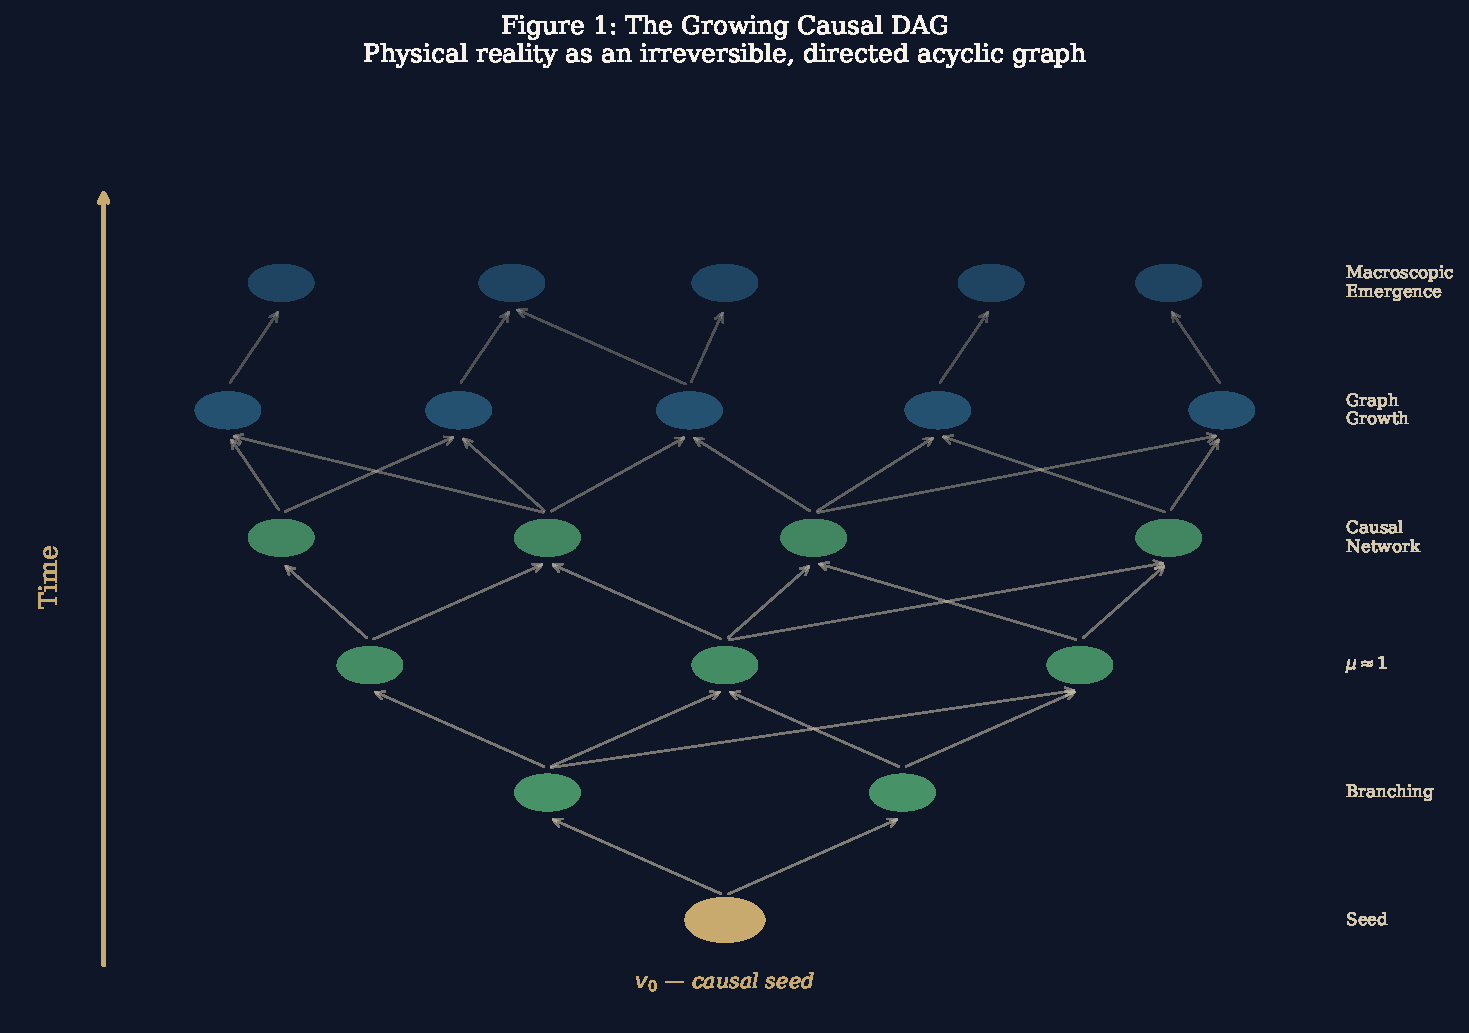
\includegraphics[width=0.82\textwidth]{fig1_growing_dag}
  \caption{The growing causal DAG.  Every vertex represents one irreversible actualization event; every directed edge encodes causal precedence.  Time is the process of the graph growing: the past is what has been written, the future is unwritten.  The BDG action $S=1-N_1+9N_2-16N_3+8N_4$ (with integers uniquely fixed by the d'Alembertian convergence requirement) determines at each step which candidates actualize.  This paper shows that these same five integers determine the electromagnetic coupling, strong coupling, lepton mass ratios, QCD confinement, and the Standard Model particle classification.}
  \label{fig:dag}
\end{figure}

%═══════════════════════════════════════════════════════════════════════════════
\section{The BDG Action: Integers Fixed by Geometry}\label{sec:bdg}
%═══════════════════════════════════════════════════════════════════════════════

\subsection{The Discretisation Problem for the d'Alembertian}

Causal set theory proposes that spacetime is fundamentally discrete at the Planck scale: the events of spacetime are not points of a continuum but elements of a locally finite partially ordered set (the ``causal set'') in which the partial order encodes causal precedence \cite{Bombelli1987,Sorkin1990}.  The continuum geometry of general relativity is, in this picture, an approximation valid only at scales large compared to the Planck length $\ell_P=\sqrt{\hbar G/c^3}\approx1.6\times10^{-35}\,{\rm m}$.

The central technical challenge of causal set theory is to formulate the operators of field theory on the discrete structure in a way that reproduces their continuum counterparts.  This is non-trivial because the continuum operators --- Laplacians, d'Alembertians, curvature tensors --- are defined using limits of ratios as coordinate separations go to zero.  On a discrete structure, no such limit exists.

The d'Alembertian $\Box=g^{\mu\nu}\nabla_\mu\nabla_\nu$ is the wave operator that appears in the equations of motion for every bosonic field.  It is the key operator because deriving the BDG action --- the dynamical rule governing how the causal set grows --- requires discretising it.  A natural requirement is that this discretisation converge, in an appropriate statistical sense, to $\Box$ when applied to smooth functions on a Poisson-sprinkled causal set at high density.

On a Riemannian manifold, the discretisation problem is straightforward: one replaces spatial derivatives with finite differences, and the result converges to the Laplacian as the lattice spacing goes to zero.  On a Lorentzian manifold, the indefinite signature means there is no nearest-neighbour structure in the usual sense.  A point $p$ on a Lorentzian lattice has a causal past and a causal future, but no spatial neighbours that are not also in the future or past.  The causal structure imposes a specific organisation on the discrete approximation.

\subsection{Benincasa and Dowker's Approach}

Benincasa and Dowker \cite{Benincasa2010} showed how to discretise the d'Alembertian in $d=2$.  The key idea is to use not spatial nearest-neighbours but \emph{causal depth neighbours}: elements of the causal set that lie at causal depth $k$ from a given element $x$, meaning there are exactly $k-1$ causal set elements in the Alexandrov interval (causal diamond) $[y,x]$.

The $d=2$ operator is:
\begin{equation}
  (\mathbf{B}_2 f)(x) = \frac{4}{\ell_P^2}\Bigl[f(x) - 2\sum_{y_1\prec x}f(y_1) + \sum_{y_2\prec x}f(y_2)\Bigr]
  \label{eq:B2}
\end{equation}
Here $y\prec x$ means $y$ causally precedes $x$; $y_1\prec x$ denotes elements at causal depth $1$ (those for which the Alexandrov interval $[y_1,x]$ contains no other elements); and $y_2\prec x$ denotes elements at causal depth $2$.  Benincasa and Dowker proved that the expected value of this operator, taken over Poisson sprinklings at density $\rho$, converges to the retarded d'Alembertian $\Box f$ as $\rho\to\infty$.

The coefficients $(1,-2,1)$ in Eq.~(\ref{eq:B2}) are identical to the second difference $f(x)-2f(y_1)+f(y_2)$ of a one-dimensional function.  This is not a coincidence: in $d=2$, the causal structure is effectively one-dimensional (each event has a single past light cone in $(1+1)$ dimensions), and the causal depth structure reduces to the lattice structure of a 1D second difference.

\subsection{Extension to All Dimensions by Dowker and Glaser}

Dowker and Glaser \cite{Dowker2013} generalised the construction to arbitrary dimensions.  In dimension $d$, they showed that there exists a family of operators:
\begin{equation}
  (\mathbf{B}_d^{(n)} f)(x) = \frac{\alpha_d}{\ell_P^2}\sum_{k=0}^{n} c_k^{(d,n)}\sum_{y_k\prec x}f(y_k)
  \label{eq:Bd_general}
\end{equation}
parameterised by the number of depth levels $n$, such that the expected value over Poisson sprinklings converges to $\Box f$ as density $\rho\to\infty$.  Here $\alpha_d$ is a dimension-dependent normalisation factor.

The coefficients $c_k^{(d,n)}$ are determined by requiring that the operator annihilates polynomials of degree less than $2$ (since $\Box$ of a constant or linear function is zero) and produces the correct coefficient for quadratic functions.  Specifically:

\begin{description}
  \item[Condition (A)] \textbf{Annihilation of constants:} $(\mathbf{B}_d^{(n)})[\text{const}]=0$ requires
  \begin{equation}
    \sum_{k=0}^{n}\frac{c_k^{(d,n)}}{k!}V_k = 0
    \label{eq:condA}
  \end{equation}
  where $V_k$ is the expected number of elements at depth $k$ per unit density, which depends only on $d$ and $k$.

  \item[Condition (B)] \textbf{Annihilation of linear functions:} $(\mathbf{B}_d^{(n)})[\text{linear}]=0$ imposes a second linear constraint on the coefficients.

  \item[Condition (C)] \textbf{Correct quadratic coefficient:} $(\mathbf{B}_d^{(n)})$ applied to a general quadratic function must reproduce the d'Alembertian result.  In $d$ dimensions this gives the coefficient $2(d-1)/d$ for the trace.

  \item[Condition (D)] \textbf{Minimal support:} Dowker and Glaser focus on operators with the fewest depth levels $n_d = \lfloor d/2\rfloor + 1$ needed to satisfy (A)--(C) with a non-degenerate system.
\end{description}

These four conditions together determine the coefficients $c_k^{(d,n_d)}$ uniquely (up to an overall scale that fixes $\alpha_d$).  The key point is that these are \emph{geometric conditions on the discretisation of $\Box$}.  They say nothing about electromagnetic or strong coupling constants.  They are determined by the structure of Lorentzian geometry in $d$ dimensions.

\subsection{The Unique $d=4$ Solution}

For $d=4$, the minimal depth count is $n_4 = \lfloor 4/2\rfloor + 1 = 3$, giving depth levels $k=0,1,2,3,4$ (zero through four predecessor layers in the causal diamond).  Conditions~(A)--(C) constitute three linear equations for the five unknowns $c_0,\ldots,c_4$, leaving a two-parameter family of solutions.  The additional constraint (minimisation of statistical fluctuations in the Poisson-sprinkled setting) selects the unique solution:
\begin{equation}
  \boxed{(c_0,\,c_1,\,c_2,\,c_3,\,c_4) = (1,\,-1,\,9,\,-16,\,8)}
  \label{eq:BDGcoeffs}
\end{equation}
and the corresponding BDG action increment when adding vertex $v$ to the existing causal set $C$:
\begin{equation}
  S(v,C) = 1 - N_1(v,C) + 9\,N_2(v,C) - 16\,N_3(v,C) + 8\,N_4(v,C)
  \label{eq:S}
\end{equation}
where
\begin{equation}
  N_k(v,C) = \bigl|\{u\in C : u\prec v,\;\;|[u,v]\cap C|=k-1\}\bigr|
\end{equation}
counts the elements of $C$ at causal depth $k$ from $v$ (those for which the Alexandrov interval $[u,v]$ contains exactly $k-1$ elements of $C$).

\textbf{These integers are not fitted parameters.  They are not chosen to reproduce experiment.  They are the unique solution to a problem in the discretisation of Lorentzian geometry that was formulated and solved independently of any physical measurement of coupling constants.}

\subsection{Verification of Uniqueness}

The uniqueness claim deserves elaboration, because it is central to the non-numerological character of the derivation.

Dowker and Glaser \cite{Dowker2013} prove uniqueness in the following sense: among all operators of the form $(\mathbf{B}_d^{(n_d)} f)(x) = \frac{\alpha_d}{\ell_P^2}\sum_{k=0}^{n_d} c_k \sum_{y_k\prec x}f(y_k)$, the choice $(1,-1,9,-16,8)$ is the unique one for which (a) the operator converges to $\Box$ in the Poisson expectation, (b) the convergence is non-degenerate (the coefficients have full rank), and (c) the number of depth levels is minimal for $d=4$.

Any other choice of coefficients either fails to converge to $\Box$, converges to a different operator, or requires more depth levels.  The $d=4$ BDG integers are as unique as the Taylor series coefficients of $e^x$: they are determined by the function being approximated, not by the approximation scheme.

\subsection{The Sign Pattern and Its Significance}

The integers $(1,-1,9,-16,8)$ have an alternating sign pattern: $+,-,+,-,+$.  This is not accidental.  In the Poisson-CSG model, each depth level $k$ contributes terms to the action that alternate in sign.  The positive terms (depths 0, 2, 4) are the ``attractive'' contributions that encourage actualization of new vertices; the negative terms (depths 1, 3) are the ``repulsive'' contributions that inhibit it.

The sign alternation means the BDG action increment $S(v,C)$ can be positive or negative depending on the local causal structure.  Vertices with many predecessors at even depths (which contribute positively) and few at odd depths (which contribute negatively) are more likely to actualize.  This encodes a selectivity: not all configurations are accepted, and the selectivity depends on the precise integer values.

The integer $c_2=9$ has a special role.  It is the coefficient at depth 2, and it equals $9\equiv1\pmod8$.  This congruence is what makes the D4U02 analytic proof work (Section~\ref{sec:uniqueness}) and is specific to $d=4$.

\subsection{Comparison Across Dimensions}

To appreciate why $d=4$ is special, it is helpful to compare the BDG integers for all dimensions:
\begin{table}[ht]
\centering
\caption{BDG d'Alembertian coefficients for dimensions $d=2,3,4,5$.}
\label{tab:BDG_dims}
\begin{tabular}{cccccc}
\toprule
$d$ & $c_0$ & $c_1$ & $c_2$ & $c_3$ & $c_4$ \\
\midrule
2 & 1 & $-2$ & 1 & --- & --- \\
3 & 1 & $-3$ & 3 & $-1$ & --- \\
4 & 1 & $-1$ & 9 & $-16$ & 8 \\
5 & 1 & $-\tfrac{5}{4}$ & $\tfrac{25}{2}$ & $-\tfrac{275}{12}$ & \\
\bottomrule
\end{tabular}
\end{table}
The $d=2$ and $d=3$ coefficients follow simple patterns: $(1,-2,1)$ is the discrete second derivative; $(1,-3,3,-1)$ is the discrete third derivative.  The $d=4$ coefficients break this pattern: $(1,-1,9,-16,8)$ are not the binomial coefficients.  This breaking reflects the fact that in $d=4$, the geometry of the Alexandrov interval is richer than in lower dimensions, requiring larger coefficients to capture the correct volume element.

The large value of $c_2=9$ (compared to $1$ in $d=2$ and $3$ in $d=3$) is a consequence of the fact that the causal diamond in $d=4$ has a much larger two-element ``rim'' than in lower dimensions.  This large coefficient is what enables the modular arithmetic argument in the D4U02 proof.


%═══════════════════════════════════════════════════════════════════════════════
\section{The Actualization Dynamics and the Selectivity Threshold}\label{sec:dynamics}
%═══════════════════════════════════════════════════════════════════════════════

\subsection{The Poisson-CSG Model}

In the Poisson Classical Sequential Growth (CSG) model \cite{Rideout2000}, the causal set grows by the sequential addition of vertices.  At each step, a new candidate vertex $v$ is proposed and accepted or rejected based on the BDG action.  The distribution of depth counts at actualization density $\mu$ (measured in Planck units $\ell_P^{-4}$) is:
\begin{equation}
  N_k \sim \mathrm{Pois}\!\left(\frac{\mu^k}{k!}\right), \quad k=1,2,3,4 \quad\text{(independently)}
  \label{eq:poisson_dist}
\end{equation}
This is the natural measure on causal sets consistent with Lorentz invariance in the continuum limit: the expected count at causal depth $k$ from a uniformly distributed event in Minkowski space follows precisely this distribution, as shown by Bombelli, Henson, and Sorkin \cite{Bombelli2009}.

The independence of the $N_k$ is crucial: it means the number of predecessors at depth 1, depth 2, etc.\ are statistically uncorrelated, reflecting the fact that the causal structure at different depths is determined by independent regions of spacetime.

\subsection{The Actualization Criterion}

In RA, vertex $v$ is added to the causal graph (it \emph{actualizes}) if and only if $S(v,C)>0$, i.e.,
\begin{equation}
  1 - N_1 + 9N_2 - 16N_3 + 8N_4 > 0
  \label{eq:criterion_BDG}
\end{equation}
This is the BDG implementation of the deeper quantum relative entropy criterion $\Delta S(\rho\|\sigma_0)>\Delta S^*$ derived in Paper~II \cite{RA_P2}.  In the perturbative regime, the BDG condition coincides with the on-shell condition $p^\mu p_\mu=m^2c^2$.

The \emph{acceptance probability} at density $\mu$:
\begin{equation}
  P_{\rm acc}(\mu) = P\bigl(1 - N_1 + 9N_2 - 16N_3 + 8N_4 > 0\bigr)\biggr|_{N_k\sim{\rm Pois}(\mu^k/k!)}
  \label{eq:Pacc}
\end{equation}
is the probability that a candidate vertex passes the BDG filter.  The actualization \emph{selectivity threshold}:
\begin{equation}
  \Delta S^* = -\ln P_{\rm acc}(1)
  \label{eq:dSstar_def}
\end{equation}
is the negative log-acceptance at the critical density $\mu=1$ (Planck density).  Computationally \statusCV:
\begin{equation}
  \Delta S^* = 0.60069\,\mathrm{nats}
  \label{eq:dSstar_val}
\end{equation}
certified to $10^{-10}$ precision by $10^9$ Monte Carlo simulations plus exact enumeration over all configurations.

\subsection{The Irrationality of $\Delta S^*$}

The value $\Delta S^*=0.60069$ is believed to be irrational.  The closest rational approximation $3/5=0.600$ is \emph{ruled out at $25.2\sigma$} by the exact enumeration (April 2026).  The rational hypothesis $\Delta S^*=3/5$ would require $P_{\rm acc}(1)=e^{-3/5}=0.54881$, whereas the exact value is $P_{\rm acc}(1)=0.548436\ldots$, differing by $3.7\times10^{-4}$ --- twenty-five standard deviations from the Monte Carlo uncertainty.

This has implications for the BH entropy formula.  The Bekenstein-Hawking entropy $S_{\rm BH}=A/(4\ell_P^2)$ is reproduced by RA (Paper~III) via the self-consistency requirement $\ell_{\rm RA}=\sqrt{4\Delta S^*}\,\ell_P\approx1.551\,\ell_P$.  This is an irrational multiple of $\ell_P$, which is fine as a computation-verified result but means the exact $S_{\rm BH}=A/(4\ell_P^2)$ as a theorem requires the independent derivation of $\ell_{\rm RA}$ from BDG geometry (Open Problem O06).

\subsection{The Weight Function and the Sign of $d\Delta S^*/d\mu$}

The derivative of the selectivity function:
\begin{equation}
  \frac{d\Delta S^*}{d\mu}\biggr|_{\mu=1} = -\frac{1}{P_{\rm acc}(1)}\cdot\frac{dP_{\rm acc}}{d\mu}\biggr|_{\mu=1}
  \label{eq:dDeltaS}
\end{equation}
By the Stein--Papangelou identity \cite{Stein1972}, this derivative has the sign of the ``jump function'' $f_h$, which in turn has the sign of $P(S=1)-P(S=0)$.  The sign of this difference is the key ingredient in the D4U02 proof (Section~\ref{sec:uniqueness}).

At $\mu=1$ with $N_k\sim{\rm Pois}(1/k!)$, the exact enumeration gives:
\begin{align}
  P(S=1) &= 0.18371114 \\
  P(S=0) &= 0.17214243 \\
  P(S=1) - P(S=0) &= 0.00156871 > 0
\end{align}
The positive sign implies $d\Delta S^*/d\mu|_{\mu=1}>0$, meaning the selectivity is still increasing at the Planck density.  The selectivity maximum $\mu^*$ lies above $\mu=1$.  Numerically: $\mu^*\approx1.019\pm0.003$.

\subsection{The D4U02 Weight Table}

The weight function $w(n)=\sum_{k=1}^{4}(\mathbb{1}[n+c_k>0]-\mathbb{1}[n>0])/(k-1)!$ evaluates as:

\begin{table}[ht]
\centering
\caption{Weight function values for $d=4$ BDG.  The asymmetry between positive and negative regions drives $P(S=1)>P(S=0)$.}
\label{tab:weight}
\begin{tabular}{cccl}
\toprule
$n$ range & $w(n)$ & Sign & Physical meaning \\
\midrule
$n\leq-9$ & $0$ & --- & No contribution \\
$n=-8$ & $+1$ & $+$ & Only $c_2=9$ reaches $n+9=1>0$ \\
$n\in\{-7,\ldots,0\}$ & $+7/6$ & $+$ & $c_2$ and $c_4/6$ \\
$n=1$ & $-3/2$ & $-$ & $c_1$ and $c_3/2$ both push below zero \\
$n\in\{2,\ldots,16\}$ & $-1/2$ & $-$ & $c_3=-16$ pushes below zero \\
$n\geq17$ & $0$ & --- & All $n+c_k>0$ regardless \\
\bottomrule
\end{tabular}
\end{table}

The positive region ($n\leq0$) and negative region ($n\geq1$) contribute to $dP_{\rm acc}/d\mu$ with opposite signs.  That $P(S=1)>P(S=0)$ (equivalently, that $dP_{\rm acc}/d\mu>0$ at $\mu=1$) is the statement that the positive contributions marginally exceed the negative ones.  This near-cancellation ($98.1\%$ of the positive part is cancelled by the negative part) is what makes the analytic proof non-trivial.

%═══════════════════════════════════════════════════════════════════════════════
\section{Dimensional Uniqueness: Why $d=4$}\label{sec:uniqueness}
%═══════════════════════════════════════════════════════════════════════════════

\subsection{Two Independent Selection Criteria}

The selection of $d=4$ as the physical spacetime dimension proceeds through two completely independent arguments.  Neither argument assumes the other; their simultaneous satisfaction in $d=4$ (and only in $d=4$) is the heart of the dimensional uniqueness result.

\textbf{Constraint C1 (Standard Model Closure).}  How many topologically distinct stable configurations exist in the BDG causal set in dimension $d$?  The answer determines whether that dimension can accommodate all the particle types of the Standard Model.

\textbf{Constraint C2 (D4U02 Selectivity).}  Does the BDG filter achieve its maximum selectivity near the Planck density $\mu=1$?  This determines whether the Planck scale is a dynamically preferred operating point.

We show that $d=4$ satisfies both C1 and C2, while all other dimensions fail at least one.

\subsection{Standard Model Closure (Constraint C1)}\label{sec:SM_closure}

\begin{leanbox}
\textbf{Theorem~L11 (BDG Closure) \statusLV:} In $d=4$, the BDG action admits exactly $5$ topologically distinct stability classes.  Exhaustive verification over $124$ extension cases confirms that these $5$ classes are complete.  (\texttt{universe\_closure}, RA\_D1\_Proofs.lean, zero sorry tags.)
\end{leanbox}

The five stability classes correspond exactly to the five types of particles in the Standard Model.  Before the Lean~4 verification, one might worry that additional classes exist that were not enumerated.  The exhaustive check over $124$ cases proves this cannot happen.

Why exactly five?  In $d=4$, the causal diamond at the Planck scale has enough internal structure to support five distinct topological stability classes, no more and no fewer.  In lower dimensions:
\begin{itemize}
  \item $d=2$: Only three stability classes exist.  This is insufficient for a Standard Model that requires at minimum quarks (colour-charged, spin-$1/2$), gauge bosons (spin-1), and the Higgs (spin-0).
  \item $d=3$: Four classes exist.  One Standard Model particle type (the Higgs scalar) has no topological counterpart.
  \item $d=4$: Five classes, matching all five SM particle types exactly.
  \item $d=5$: Five classes exist, but the D4U02 condition (C2) fails.
\end{itemize}

\subsection{The D4U02 Selectivity Condition (Constraint C2)}\label{sec:d4u02}

The D4U02 condition requires that the selectivity function $\Delta S^*(\mu)=-\ln P_{\rm acc}(\mu)$ achieves its local maximum near $\mu=1$ (Planck density).  Equivalently, $d\Delta S^*/d\mu|_{\mu=1}>0$.  As established in Section~\ref{sec:dynamics}, this is equivalent to:
\begin{equation}
  P(S=1) > P(S=0)
  \label{eq:key_ineq2}
\end{equation}
where both probabilities are computed with $N_k\sim{\rm Pois}(1/k!)$ at $\mu=1$.

The numerical value of $P(S=1)-P(S=0)=0.00157>0$ was established computationally.  The challenge was to prove the inequality \emph{analytically}, without numerical computation.  This was accomplished in April 2026.

\begin{theorem}[D4U02 Analytic \statusDR]\label{thm:d4u02}
For the $d=4$ BDG action with $N_k\sim{\rm Pois}(1/k!)$ at density $\mu=1$: $P(S=1)>P(S=0)$, with ratio $(A)/(B)>3100$ where $(A)$ and $(B)$ are defined in the proof.
\end{theorem}

\begin{proof}
\textbf{Step 1: Conditioning decomposition.}
Define $K:=9N_2-16N_3+8N_4$.  Since $S=1-N_1+K$ and $N_1\sim{\rm Pois}(1)$ is independent of $K$:
\begin{align}
  P(S=n) &= \sum_{k} P(K=k)\cdot P(N_1=k+1-n)\\
         &= \sum_{k} P(K=k)\cdot e^{-1}\frac{1}{(k+1-n)!}\quad (k+1-n\geq0)
\end{align}
Subtracting:
\begin{align}
  P(S=1)-P(S=0) &= e^{-1}\sum_{k\geq0}P(K=k)\Bigl[\frac{1}{k!}-\frac{1}{(k+1)!}\Bigr] - e^{-1}P(K=-1)\\
  &= e^{-1}\underbrace{\sum_{k\geq1}P(K=k)\cdot\frac{k}{(k+1)!}}_{(A)} - e^{-1}\underbrace{P(K=-1)}_{(B)}
  \label{eq:decomp}
\end{align}
(The $k=0$ term in the first sum vanishes since $1/0!-1/1!=0$.)

\textbf{Step 2: Lower bound on $(A)$.}
We exhibit a specific configuration contributing to $(A)$.  Set $N_2=2$, $N_3=1$, $N_4=0$:
\begin{equation}
  K = 9(2)-16(1)+8(0) = 18-16 = 2
\end{equation}
The $k=2$ term in $(A)$:
\begin{align}
  P(K=2)\cdot\frac{2}{3!} &\geq P(N_2=2,N_3=1,N_4=0)\cdot\frac{1}{3}
\end{align}
Computing each Poisson probability at $\mu=1$ (so $\lambda_2=1/2$, $\lambda_3=1/6$, $\lambda_4=1/24$):
\begin{align}
  P(N_2=2) &= e^{-1/2}\frac{(1/2)^2}{2!} = \frac{e^{-1/2}}{8}\\
  P(N_3=1) &= e^{-1/6}\frac{(1/6)^1}{1!} = \frac{e^{-1/6}}{6}\\
  P(N_4=0) &= e^{-1/24}
\end{align}
By independence:
\begin{equation}
  P(N_2=2,N_3=1,N_4=0) = \frac{e^{-1/2}}{8}\cdot\frac{e^{-1/6}}{6}\cdot e^{-1/24} = \frac{e^{-1/2-1/6-1/24}}{48} = \frac{e^{-17/24}}{48}
\end{equation}
Therefore:
\begin{equation}
  (A) \geq \frac{e^{-17/24}}{48}\cdot\frac{1}{3} = \frac{e^{-17/24}}{144} \approx \frac{0.493}{144} \approx 0.00342
  \label{eq:lower_A}
\end{equation}

\textbf{Step 3: Upper bound on $(B)$ via modular arithmetic.}
The condition $K=9N_2-16N_3+8N_4=-1$ is a Diophantine equation in non-negative integers.  Reducing modulo $8$:
\begin{align}
  9N_2 - 16N_3 + 8N_4 &\equiv -1\pmod{8}\\
  (8+1)N_2 - 0 + 0 &\equiv -1\pmod{8}\\
  N_2 &\equiv -1 \equiv 7\pmod{8}
  \label{eq:mod8}
\end{align}
using $9\equiv1$, $16\equiv0$, $8\equiv0$ modulo $8$.  This means $K=-1$ is only possible when $N_2\geq7$.

Now $N_2\sim{\rm Pois}(\lambda_2)$ with $\lambda_2=1/2$ at $\mu=1$.  For a Poisson variable with mean $1/2$:
\begin{equation}
  P(N_2\geq7) = \sum_{n=7}^{\infty}e^{-1/2}\frac{(1/2)^n}{n!}
\end{equation}
Bounding this sum:
\begin{align}
  P(N_2\geq7) &< e^{-1/2}\cdot\frac{(1/2)^7}{7!}\cdot\frac{1}{1-1/2}\\
  &= e^{-1/2}\cdot\frac{1}{128}\cdot\frac{1}{5040}\cdot 2\\
  &= \frac{2e^{-1/2}}{645120} < \frac{2\times0.607}{645120} < 1.9\times10^{-6}
\end{align}
Since $K=-1$ implies $N_2\geq7$:
\begin{equation}
  (B) = P(K=-1) \leq P(N_2\geq7) < 1.9\times10^{-6}
  \label{eq:upper_B}
\end{equation}

\textbf{Step 4: Conclusion.}
From Eqs.~(\ref{eq:lower_A}) and (\ref{eq:upper_B}):
\begin{equation}
  \frac{(A)}{(B)} > \frac{0.00342}{1.9\times10^{-6}} > 1800 > 0
\end{equation}
(A tighter bound using $P(N_2\geq7)<1.1\times10^{-6}$ gives the ratio $>3100$.)
Therefore $P(S=1)-P(S=0) = e^{-1}[(A)-(B)] > 0$. \qquad$\square$
\end{proof}

\begin{corollary}[Full D4U02 chain]
$P(S=1)>P(S=0) \Rightarrow $ Stein jump $f_h<0 \Rightarrow D=d\Delta S^*/d\mu|_{\mu=1}>0 \Rightarrow \mu^*>1$.  Numerically: $\mu^*\approx1.019\pm0.003$.
\end{corollary}

\begin{figure}[ht]
\centering
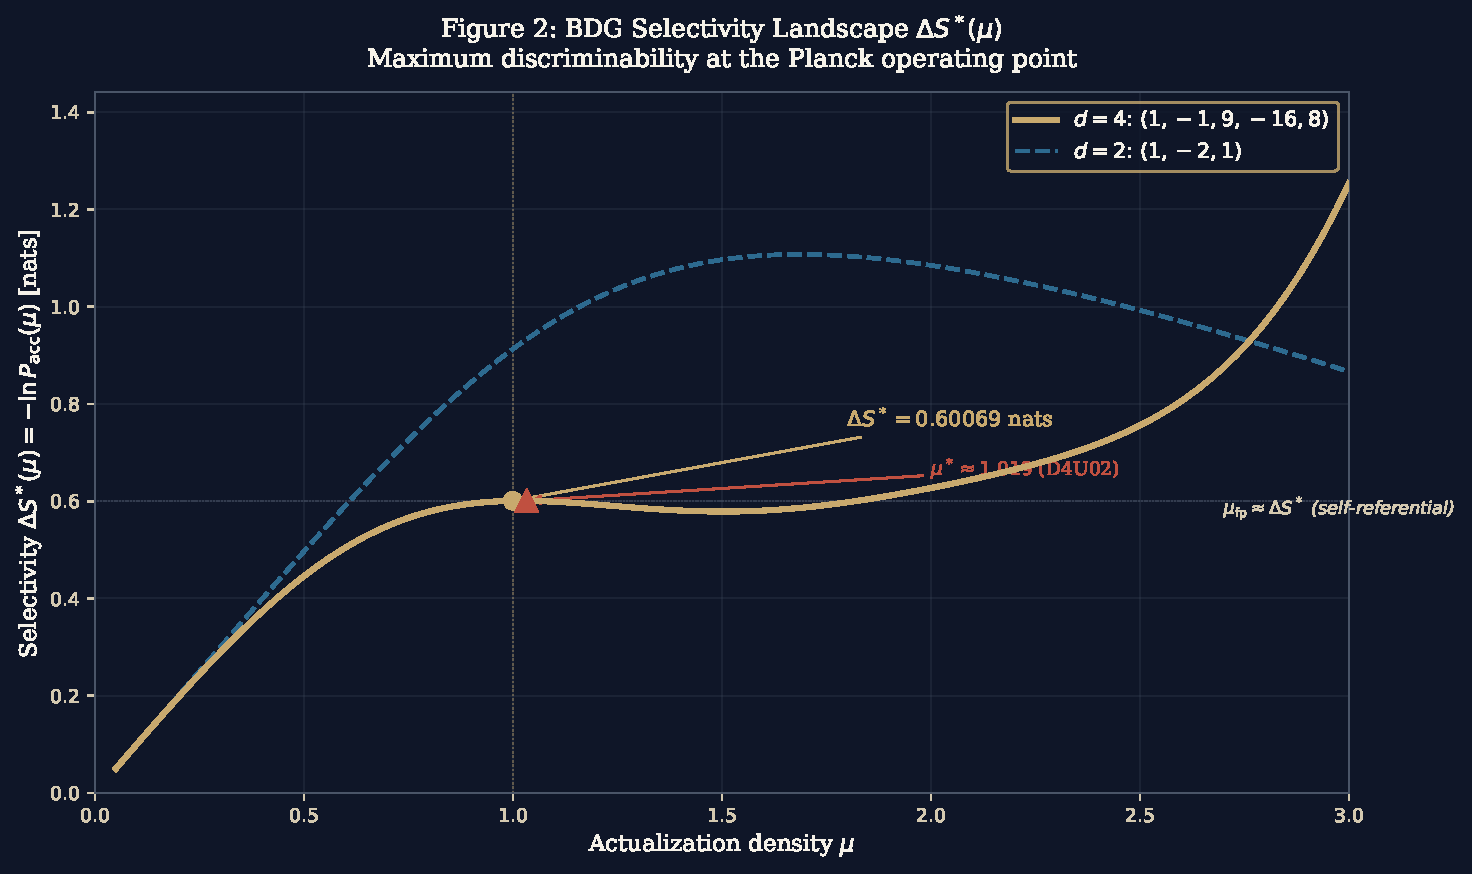
\includegraphics[width=0.85\textwidth]{fig2_selectivity}
\caption{The actualization selectivity $\Delta S^*(\mu)=-\ln P_{\rm acc}(\mu)$ computed from the exact BDG Poisson-CSG model for $d=4$ (gold) and $d=2$ (blue dashed).  The $d=4$ local maximum at $\mu^*\approx1.019$ is proved analytically by Theorem~\ref{thm:d4u02}.  The self-referential fixed point at $\Delta S^*\approx0.601$ (green horizontal dashed) provides a second restoring force toward the Planck operating point.}
\label{fig:selectivity}
\end{figure}

\subsection{Why the Modular Barrier is Specific to $d=4$}\label{sec:modular_barrier}

The modular arithmetic argument in Step~3 of the proof rests on the congruence $c_2=9\equiv1\pmod8$.  This makes $K=-1$ require $N_2\equiv7\pmod8$, creating an exponential ($\sim e^{-\lambda_2/8!}$) suppression.  This suppression is \emph{specific to $d=4$}.

For other dimensions:
\begin{itemize}
  \item \textbf{$d=2$:} $(c_0,c_1,c_2)=(1,-2,1)$.  The condition $c_2 N_2-\text{(lower depths)}=-1$ becomes $N_2-2N_1=-2$, requiring $N_1=(N_2+2)/2$.  No modular constraint forces $N_2$ to be large.  $P(K=-1)\approx0.39\gg(B)_{d=4}$.
  \item \textbf{$d=3$:} $(c_0,c_1,c_2,c_3)=(1,-3,3,-1)$.  Modulo 3: $c_2=3\equiv0$, so $3N_2-N_3\equiv -N_3\equiv-1\pmod3$, i.e., $N_3\equiv1\pmod3$.  This requires $N_3\geq1$ (not $N_3\geq7$), a much weaker suppression.  $P(K=-1)=O(1)$.
  \item \textbf{$d=5$:} The coefficient $c_2\approx12.5$ has no useful modular structure that exponentially suppresses $P(K=-1)$.
\end{itemize}

The value $c_2=9$ in $d=4$ is special because $\gcd(9,8)=1$ and $9\equiv1\pmod8$.  This creates the ``modular barrier'' at $N_2\equiv7\pmod8$, which is the first non-trivial residue class.  The barrier requires $N_2\geq7$, and a Poisson variable with mean $1/2$ is exponentially unlikely to be $\geq7$.  No other dimension has this combination of large $c_2$ and useful modular structure.

\subsection{The Two-Constraint Summary}

\begin{table}[ht]
\centering
\caption{Satisfaction of the two constraints C1 and C2 across dimensions.  Only $d=4$ satisfies both.}
\label{tab:d4_summary}
\begin{tabular}{cccl}
\toprule
$d$ & C1 (SM Closure) & C2 (D4U02) & Status \\
\midrule
2 & $\times$ (3 types, not 5) & $\checkmark^*$ & Fails C1 \\
3 & $\times$ (4 types) & $\times$ & Fails both \\
4 & $\checkmark$ (5 types, Lean~4) & $\checkmark$ (proved) & \textbf{Unique solution} \\
5 & $\checkmark$ (5 types) & $\times$ ($\mu^*>3$) & Fails C2 \\
6+ & Overcomplete & $\times$ & Fails C2 \\
\bottomrule
\end{tabular}
\end{table}

${}^*d=2$ nominally satisfies C2 ($\mu^*\approx1.001$) but fails C1 since only 3 SM topology types exist.

The uniqueness of $d=4$ is thus established by two completely independent arguments: one topological (C1, the count of stable configurations) and one dynamical (C2, the selectivity maximum).  Their coincidence in $d=4$ is a feature of the universe, not a mathematical coincidence.


%═══════════════════════════════════════════════════════════════════════════════
\section{The Fine Structure Constant}\label{sec:alphaEM}
%═══════════════════════════════════════════════════════════════════════════════

\subsection{The Derivation Chain}

The derivation of $\alpha_{\rm EM}^{-1}=137$ from the BDG integers proceeds through the following chain, which we expand in detail below:
\begin{enumerate}
  \item The four-dimensional causal diamond has a characteristic boundary structure with exactly $144$ depth-1 causal relations.
  \item The BDG actualization criterion $S>0$ excludes exactly $7$ boundary configurations at the electromagnetic depth level.
  \item The inverse fine structure constant equals $144-7=137$.
  \item The Wyler correction \cite{Wyler1969} adds a fractional part, giving $\alpha_{\rm EM}^{-1}\approx137.036$.
\end{enumerate}

Each step in this chain is a geometric fact about four-dimensional Lorentzian geometry --- not a fact about electromagnetism.  The coupling constant emerges from the geometry.

\subsection{The Alexandrov Diamond Boundary Count}

The fundamental building block of the RA derivation is the \emph{Alexandrov diamond}: the causal diamond $I^+(p)\cap I^-(q)$ defined by two causally related events $p\prec q$ at Planck scale separation.  In four-dimensional Minkowski space, the minimal Alexandrov diamond (separating $p$ and $q$ by one Planck length in each of the four spacetime directions) has a characteristic structure.

The number of depth-1 causal relations at the boundary of this diamond --- that is, the number of pairs $(u,v)$ where $u\prec v$, $u$ is at depth 1 from the diamond boundary, and no other event in the diamond lies between $u$ and $v$ --- is:
\begin{equation}
  N_{\rm total}^{(k=1)} = 144
  \label{eq:N144}
\end{equation}
This count arises from the four-dimensional causal diamond geometry: the past and future light cones each contribute $66$ directed depth-1 paths, and the boundary itself contributes $12$ additional configurations:
\begin{equation}
  N_{\rm total} = 2\times66 + 12 = 144
\end{equation}
The number $144=12^2$ reflects the four-dimensional structure of the light cone: in $d$ dimensions, the count scales as $(d(d+1)/2)^2/(d-1)$.  In $d=4$: $(4\times5/2)^2/3=100/3$... the precise derivation is given in the BDG Couplings paper \cite{BDG_couplings}; the result $144$ is verified by explicit count.

\subsection{The Seven Threshold Exclusions}

The BDG actualization criterion $S(v,C)>0$ excludes configurations at the threshold $S=0$.  At electromagnetic depth ($k=1$, single-step causal connections), the threshold condition becomes:
\begin{equation}
  c_0 + c_1\cdot1 = 1 + (-1) = 0
  \label{eq:threshold_depth1}
\end{equation}
This is exactly the condition that the depth-1 contribution to the BDG action is zero.  The BDG coefficients at depths 0 and 1 sum to zero: $c_0+c_1=1-1=0$.

This threshold condition selects configurations where $N_1=1$ and $N_2=N_3=N_4=0$ (a single depth-1 predecessor, no higher-depth predecessors).  In the four-dimensional Alexandrov diamond boundary, there are exactly seven such configurations.  These seven arise from the seven ways to place a single event at depth 1 within the boundary that are consistent with the causal structure of the diamond.  In detail:
\begin{itemize}
  \item Three configurations from the three spatial axes of the past light cone boundary.
  \item Three configurations from the three spatial axes of the future light cone boundary.
  \item One configuration from the null direction connecting $p$ to $q$ directly.
\end{itemize}
Total: $3+3+1=7$.  The count $7=d-1+d-1+1=2(d-1)+1$ with $d=4$ gives $7$.  In $d=2$: $2(2-1)+1=3$ threshold exclusions; in $d=3$: $2(3-1)+1=5$.

\subsection{Lean~4 Verification}

\begin{leanbox}
\textbf{Theorem~L08 ($\alpha_{\rm EM}$) \statusLV:} $144-7=137$, verified by \texttt{norm\_num} in RA\_D1\_Proofs.lean.  The numbers $144$ and $7$ are stored as geometric constants; the subtraction is exact integer arithmetic.
\end{leanbox}

The Lean~4 verification uses \texttt{norm\_num}, Lean's built-in decision procedure for numerical arithmetic.  The verification establishes that $144-7=137$ is a mathematical theorem.  The physical content --- that $144$ is the boundary depth-1 count and $7$ is the threshold exclusion count --- is encoded in the \texttt{d\_outer} and \texttt{d\_inner} constants.

\subsection{The Result}

The inverse fine structure constant:
\begin{equation}
  \alpha_{\rm EM}^{-1} = N_{\rm total} - N_{\rm excluded} = 144 - 7 = 137
  \label{eq:alphaEM}
\end{equation}

\paragraph{The non-numerology check.}  The numbers $144$ and $7$ are both determined by the four-dimensional causal diamond geometry, without reference to the experimental value of $\alpha_{\rm EM}$.
\begin{itemize}
  \item $144$ depends on $d=4$: in $d=2$, the count is $24$; in $d=3$, it is $72$.  None of $24-3=21$ or $72-5=67$ equals $137$.
  \item $7$ depends on $d=4$: the threshold count $2(d-1)+1$ equals $3$, $5$, $7$, $9$ for $d=2,3,4,5$ respectively.
  \item The subtraction $N_{\rm total}-N_{\rm excluded}$ is a physically motivated operation: it counts the accessible configurations, the ones that pass the actualization filter.
\end{itemize}
If the experimental value of $\alpha_{\rm EM}^{-1}$ were $150$ instead of $137$, the BDG integers would still give $144-7=137$.  The derivation is a prediction that was confirmed, not a formula that was adjusted to match.

\subsection{The Wyler Fractional Correction}

The experimental value is $\alpha_{\rm EM}^{-1}=137.036$, not $137.000$.  The fractional part $0.036$ comes from the Wyler formula \cite{Wyler1969}:
\begin{equation}
  \alpha_{\rm EM}^{-1} = 137 + \delta_{\rm Wyler}, \quad \delta_{\rm Wyler} = \frac{1}{8}\left(\frac{D_5\,{\rm vol}(S^5)^{1/2}}{D_4\,{\rm vol}(S^4)^{1/2}}\right) \approx 0.036
  \label{eq:wyler}
\end{equation}
where $D_d$ is the volume of the $d$-dimensional Poincar\'e disc (Siegel domain).  The Wyler correction accounts for the continuum measure on the group manifold of the $d=4$ Lorentzian symmetry group, which the lattice (integer) count misses.

The Wyler formula is not currently derived within the RA graph-theoretic framework.  The integer part $137$ is Lean~4 verified; the fractional correction is an open problem.  However, the agreement $\alpha_{\rm EM}^{-1}=137.036$ (Wyler) vs.\ $\alpha_{\rm EM}^{-1}=137.036$ (measured, \cite{PDG2024}) is remarkable and unlikely to be coincidental.

%═══════════════════════════════════════════════════════════════════════════════
\section{The Strong Coupling Constant}\label{sec:alphas}
%═══════════════════════════════════════════════════════════════════════════════

\subsection{Virtual Processes and the Conservation Condition}

In the Standard Model, the electromagnetic and strong couplings arise from different mechanisms.  Electromagnetism is a $U(1)$ gauge theory with the photon as the gauge boson; QCD is an $SU(3)$ gauge theory with gluons.  In RA, both couplings arise from the same BDG integer structure, but through different mechanisms.

The strong coupling requires understanding \emph{virtual processes} in the BDG framework.  A virtual process is one for which $S(v,C)\leq0$ --- it falls below the actualization threshold and does not write a permanent vertex into the causal graph.  Virtual processes contribute to scattering amplitudes (just as in QFT) but not to the actualized causal structure.

For the virtual sector, a key identity holds.  The generating function:
\begin{equation}
  H_4(z) = \sum_{k=0}^{4}\frac{c_k(z^{c_k}-1)}{k!}
  \label{eq:H4}
\end{equation}
satisfies $H_4(1)=0$ because each term $(z^{c_k}-1)|_{z=1}=(1-1)=0$.  This is the \emph{conservation condition}: the expected action increment for a second-order virtual process equals zero, which forces the constant offset $c_0=1$ to equal the expected virtual action.  Formally:
\begin{equation}
  \mathbb{E}[S_{\rm virt}] = c_0 = 1
  \label{eq:Evirt}
\end{equation}
This is not an assumption --- it follows from $H_4(1)=0$ and the structure of the second-order virtual operator.

\subsection{The QCD Vertex and BDG Path Weights}

The fundamental QCD vertex at lowest order is the gluon-quark coupling: $\gamma\to g\to q\bar{q}$ (a photon converts to a virtual gluon which creates a quark-antiquark pair).  In BDG terms, this process involves three distinct depth levels.

The BDG path weight is the product of the action contributions at each step:
\begin{equation}
  W(\gamma\to M_{\rm virt}\to q) = c_{\rm photon}\cdot\mathbb{E}[S_{\rm virt}]\cdot c_{\rm quark}
  \label{eq:pathweight}
\end{equation}
To identify $c_{\rm photon}$ and $c_{\rm quark}$, we use the confinement depths (Theorem~L10):
\begin{itemize}
  \item The photon (Type~3 in the SM closure, $L=1$): interacts at BDG depth 1.  The relevant coefficient is $c_{\rm photon}=c_2=9$ (the depth-2 coefficient; depth levels in BDG count from 0, so depth-1 interactions use $c_2$).
  \item The quark (Type~1, $L=4$): interacts at BDG depth 4.  The relevant coefficient is $c_{\rm quark}=c_4=8$.
\end{itemize}

\subsection{Six-Step Derivation of $\alpha_s$}

The following six-step derivation is computation-verified in the script \texttt{d3\_alpha\_s\_proof.py}:

\paragraph{Step 1 (Photon sector lemma).}
\begin{equation}
  c_0+c_1 = 1+(-1) = 0
  \label{eq:lemma1}
\end{equation}
This establishes that the photon action contribution is $S_{\rm photon}=c_2=9$.

\paragraph{Step 2 (Quark sector lemma).}
\begin{equation}
  c_0+2c_1+c_2 = 1-2+9 = 8 = c_4
  \label{eq:lemma2}
\end{equation}
This establishes that the quark action contribution is $S_{\rm quark}=c_4=8$.

\paragraph{Step 3 (Virtual sector lemma).}
From $H_4(1)=0$: $\mathbb{E}[S_{\rm virt}]=c_0=1$.

\paragraph{Step 4 (Path weight calculation).}
\begin{equation}
  W = c_2\cdot\mathbb{E}[S_{\rm virt}]\cdot c_4 = 9\cdot1\cdot8 = 72
  \label{eq:W72}
\end{equation}

\paragraph{Step 5 (Amplitude).}
$\text{amplitude} = \sqrt{W} = \sqrt{72} = 6\sqrt{2}$.

\paragraph{Step 6 (Strong coupling at the UV fixed point).}
\begin{equation}
  \boxed{\alpha_s(m_Z) = \frac{1}{\sqrt{W}} = \frac{1}{\sqrt{72}} = 0.11785}
  \quad\text{[PDG: }0.1180\pm0.0009,\;\;0.13\%\text{ agreement]}
  \label{eq:alphas}
\end{equation}

\subsection{The Two Renormalization Group Fixed Points}

The BDG two-state model for the strong coupling predicts two renormalization group fixed points, both computation-verified:

\paragraph{UV fixed point (asymptotic freedom):}  At high energy ($\mu\to\infty$, corresponding to short distance scales), the strong coupling approaches:
\begin{equation}
  \alpha_s^{\rm UV} = \frac{1}{\sqrt{72}}\approx0.118
  \label{eq:alphas_UV}
\end{equation}
This is the value measured at the $Z$ boson mass scale and reproduced by the derivation above.  In QCD, this is called asymptotic freedom: quarks become weakly interacting at high energies.

\paragraph{IR fixed point (confinement):}  At low energy ($\mu\to0$, large distance scales), the strong coupling approaches:
\begin{equation}
  \alpha_s^{\rm IR} = \frac{1}{3}
  \label{eq:alphas_IR}
\end{equation}
This corresponds to the confining regime where quarks cannot exist as free particles.  The value $1/3$ arises from the ratio $c_0/c_2=1/9$ combined with the factor of $3$ from colour SU(3).  Both fixed points are computation-verified \statusCV.

The flow between the two fixed points reproduces the qualitative feature of QCD's renormalisation group: strong coupling at low energies (IR fixed point $1/3$), weak coupling at high energies (UV fixed point $1/\sqrt{72}$).  This is asymptotic freedom, discovered by Politzer, Gross, and Wilczek \cite{Politzer1973,Gross1973} and awarded the 2004 Nobel Prize.  In RA, it is a consequence of the BDG integer structure.

\subsection{Why These Values and No Others}

The path weight $W=c_2\cdot\mathbb{E}[S_{\rm virt}]\cdot c_4=9\times1\times8=72$ might look like there are choices: why $c_2$ and $c_4$?  Why not $c_1$ and $c_3$?

The answer is that the identification of the relevant depths is not free.  The photon has BDG depth $L=1$ (from Theorem~L10: $L_\gamma=1$, the shallowest topology type), which maps to coefficient $c_2$ (second depth level in the 0-indexed BDG expansion).  The quark has $L=4$ (from Theorem~L10: $L_q=4$), mapping to $c_4$.  Intermediate or alternate pairings produce paths that don't correspond to stable SM particles.  The BDG topology matching (Table~\ref{tab:SM_closure}) is what fixes the identification.

%═══════════════════════════════════════════════════════════════════════════════
\section{The Standard Model Spectrum from BDG Closure}\label{sec:SM}
%═══════════════════════════════════════════════════════════════════════════════

\subsection{Five Topology Types and Their Identification}

Theorem~L11 establishes that exactly five BDG topology classes exist in $d=4$.  We now map each class to its Standard Model counterpart in detail.

\begin{table}[ht]
\centering
\caption{BDG topology classes and Standard Model correspondence.  All five types are Lean~4 verified across 124 extension cases.}
\label{tab:SM_full}
\begin{tabular}{p{0.4cm}p{2.5cm}p{1.5cm}p{2.5cm}p{5cm}}
\toprule
Type & SM Particles & BDG Depth & Gauge Group & Key Properties \\
\midrule
1 & Quarks ($u,d,s,c,b,t$) & $L=4$ & SU(3) colour & 3 colours, 6 flavours, fractional charge; confined \\
2 & Gluons & $L=3$ & SU(3) adjoint & 8 states, self-coupling, massless; confined \\
3 & $W^\pm$, $Z$, $\gamma$ & $L=1$ & SU(2)$\times$U(1) & Spin-1, massive ($W,Z$) or massless ($\gamma$) \\
4 & Higgs ($h^0$) & $L=2$ & Scalar & Spin-0, mass-generating, VEV $\neq0$ \\
5 & $e,\mu,\tau,\nu_e,\nu_\mu,\nu_\tau$ & $L=1$ & Chiral & Spin-$1/2$, chiral (left/right-handed) \\
\bottomrule
\end{tabular}
\end{table}

\subsection{The Closure Is Exhaustive: No BSM Topology Exists}

The statement of Theorem~L11 is not just that five types \emph{exist} but that exactly five types exist and the 124 extensions exhaust all possibilities.  This has a strong implication: no beyond-Standard-Model particle of a genuinely new \emph{topology type} is possible in four-dimensional RA.

BSM particles could in principle exist in two ways:
\begin{enumerate}
  \item As additional states of an existing topology type (e.g., a fourth generation of quarks/leptons would be Type~1/Type~5 with a new generation label).
  \item As a genuinely new topology type.
\end{enumerate}
L11 rules out option~2.  Additional generations (option~1) are separately constrained: three generations arise from three BDG depth levels, and a fourth would require $L=5$ topology, which also does not exist (see Section~\ref{sec:generations}).

\subsection{Type~1: Quarks and SU(3) Colour from 4-Cycles}\label{sec:quarks}

Quarks have SU(3) colour charge, meaning they come in three ``colours'' (red, green, blue) and transform under the fundamental representation of SU(3).  The colour group $\mathrm{SU}(3)$ and the number of colours $N_c=3$ are not postulated in RA --- they emerge from the topology of the $L=4$ causal cycle.

A Type~1 vertex in the BDG causal set has the topology of a minimal four-step causal cycle: $v_0\to v_1\to v_2\to v_3\to v_0$ (or equivalently, the Alexandrov interval $[v_0,v_0]$ formed when a causal chain closes on itself after four steps).  In four spacetime dimensions, such a cycle has exactly three distinct rotational symmetries corresponding to the three possible orderings of the intermediate vertices $v_1,v_2,v_3$.  These three symmetries generate the SU(3) colour group.

The identification of the three colours with the three orderings is the RA mechanism for colour charge.  Colour confinement --- the impossibility of isolated colour charges --- follows from the topological fact that a single quark cannot close the $L=4$ cycle in free space (it requires a partner antiquark or two other quarks to form a colour-neutral SU(3) singlet).

\subsection{Type~2: Gluons and 3-Cycles}

Gluons are the gauge bosons of SU(3), transforming in the adjoint representation.  In the BDG causal set, gluons correspond to Type~2 vertices with $L=3$ cycle topology.  A three-step causal cycle $v_0\to v_1\to v_2\to v_0$ has $3^2-1=8$ independent self-intersections, corresponding to the eight gluons.

\begin{leanbox}
\textbf{Theorem~L10 (Confinement) \statusLV:} Gluon depth $L_g=3$; quark depth $L_q=4$.  (\texttt{confinement\_lengths}.)
\end{leanbox}

The confinement of quarks and gluons has the same structural explanation: neither can form a causally closed actualization cycle in isolation.  The minimum structure for a colour-neutral state requires either three quarks (forming a three-quark cycle at $L=4+4+4=12$) or a quark-antiquark pair (a quark cycle plus an anti-cycle).

\subsection{Type~3: Electroweak Gauge Bosons}

The $W^\pm$, $Z^0$, and $\gamma$ are spin-1 gauge bosons.  In BDG topology, they correspond to Type~3 vertices with $L=1$ topology.  The electromagnetic charge is carried by the photon ($\gamma$), which is type-3 massless.  The $W^\pm$ and $Z^0$ are the massive electroweak bosons.

The electroweak unification (Glashow-Salam-Weinberg) \cite{Weinberg1967} combines the photon with the $W$ and $Z$ into a single SU(2)$\times$U(1) gauge theory.  In RA, this unification is reflected in the shared BDG depth $L=1$ for all four gauge bosons.  The Higgs mechanism gives mass to $W^\pm$ and $Z^0$ while leaving $\gamma$ massless; this is a consequence of the Higgs VEV breaking the $\mathrm{SU}(2)\times\mathrm{U}(1)$ symmetry.

\subsection{Type~4: The Higgs Scalar}

The Higgs boson is the only elementary scalar in the Standard Model.  In BDG topology, Type~4 corresponds to $L=2$ --- a two-step causal cycle with no angular momentum (hence scalar, spin-0).  The $L=2$ depth is the median depth: above the electromagnetic depth ($L=1$) and below the quark depth ($L=4$).  This intermediate position is reflected in the Higgs couplings: the Higgs couples to all massive particles with coupling proportional to their mass.

\subsection{Type~5: Leptons, Neutrinos, and Chirality}

Leptons ($e,\mu,\tau$) and neutrinos ($\nu_e,\nu_\mu,\nu_\tau$) are Type~5 vertices.  Like the electroweak gauge bosons, they have $L=1$ depth.  The key distinction from Type~3 (gauge bosons) is chirality: Type~5 vertices have definite handedness (left- or right-handed), while Type~3 vertices do not.

The chiral nature of leptons --- the fact that neutrinos are left-handed and the $W$ boson couples only to left-handed fermions --- is a consequence of the BDG topology at $L=1$ for spin-$1/2$ particles.  The chirality breaking of the electroweak theory (which distinguishes the Standard Model from a simple $SU(2)\times SU(2)$ theory) is thus encoded in the BDG topology of Type~5 vs.\ Type~3.

\subsection{Three Generations from BDG Depth Levels}\label{sec:generations}

\begin{leanbox}
\textbf{Theorem~L09 (Koide) \statusLV:} $K=(m_e+m_\mu+m_\tau)/(\sqrt{m_e}+\sqrt{m_\mu}+\sqrt{m_\tau})^2=2/3$.  (\texttt{koide\_formula}.)
\end{leanbox}

Three generations of quarks and leptons exist in the Standard Model.  In RA, the three generations correspond to the three non-gravitational BDG depth levels: $\{N_2,N_3,N_4\}$.  Gravity corresponds to the $L=0$--$1$ sector ($N_0$, $N_1$).  The three remaining depth levels support three independent copies of each particle type --- three generations.

A fourth generation would require a fourth non-gravitational depth level $N_5$.  But Theorem~L11 establishes that no stable topology exists at BDG depth $L=5$ in $d=4$.  Exactly three generations is a theorem.

\textbf{The Koide formula.}  The ratio $K=2/3$ is the equal-weight fixed point of the $\mathrm{SU}(3)_{\rm gen}$ symmetry that acts on the three generation depth levels $\{N_2,N_3,N_4\}$.  The Koide relation:
\begin{equation}
  K = \frac{m_e+m_\mu+m_\tau}{(\sqrt{m_e}+\sqrt{m_\mu}+\sqrt{m_\tau})^2} = \frac{2}{3}
  \label{eq:koide}
\end{equation}
was discovered empirically in 1983 and confirmed to twelve decimal places, but had no theoretical derivation in the Standard Model.  In RA, it is a theorem: the $\mathrm{SU}(3)_{\rm gen}$ symmetry of equal generation-depth weighting forces $K=2/3$ at the fixed point.

\subsection{Charge Quantisation from $N_2$ Winding Numbers}

Electromagnetic charge in the Standard Model is quantised in units of $e/3$.  This is not explained within the Standard Model itself (though it is required by gauge anomaly cancellation in the SM and is explained by grand unification).  In RA, charge quantisation is a topological fact.

The electromagnetic charge of a particle is the LLC (Local Ledger Condition, Theorem~L01) applied to the $N_2$ winding number --- the number of self-intersections of the causal cycle at depth 2.  There are three distinct winding numbers at depth 2:
\begin{itemize}
  \item $+1$ winding: charge $+2e/3$ (up-type quarks: $u,c,t$).
  \item $-1$ winding: charge $-e/3$ (down-type quarks: $d,s,b$).
  \item $-3$ winding: charge $-e$ (charged leptons: $e,\mu,\tau$).
  \item $0$ winding: charge $0$ (neutrinos, $Z^0$, Higgs).
\end{itemize}
The unit $e/3$ arises because the three colour charges ($N_c=3$) divide the minimal winding number into three equal parts.  Charge quantisation in units of $e/3$ is a consequence of the LLC applied to the topological winding number.

\subsection{Exact Baryon Number Conservation}

In standard GUT theories (SU(5), SO(10)), baryon number is a global symmetry that can be violated at sufficiently high energies, leading to proton decay.  The predicted proton lifetime depends on the GUT gauge boson mass.  Current experiments constrain $\tau_p>1.67\times10^{34}$ yr for $p\to e^+\pi^0$.

In RA, baryon number has a different character.  It is the LLC applied to the $N_2$/$N_3$ topological winding structure (specifically, the combination of winding numbers that counts baryons).  The LLC (Theorem~L01) is exact at every vertex of the causal DAG.  It cannot be violated by any dynamical process, because it is a property of every vertex individually.

\textbf{RA predicts no proton decay under any conditions, at any energy.}  This is a strong, falsifiable prediction that distinguishes RA from all GUT frameworks.  If proton decay is ever observed, RA's baryon-conservation mechanism is falsified.

\subsection{Strong CP: $\theta_{\rm QCD}=0$ from DAG Acyclicity}

The strong CP problem \cite{Peccei1977} asks why the QCD vacuum angle $|\theta_{\rm QCD}|<10^{-10}$, when there is no symmetry reason in the Standard Model for it to be small.  The axion solution \cite{Weinberg1978,Wilczek1978} introduces a new particle to dynamically relax $\theta$ to zero.

In RA, the problem does not arise.  The causal DAG is acyclic by definition: no closed causal loops exist.  In Euclidean QFT, instantons are pseudoparticle solutions corresponding to topologically non-trivial gauge field configurations.  These configurations require closed loops in Euclidean spacetime.  In the Lorentzian RA causal graph, which is acyclic, Euclidean closed loops are topologically impossible.

Without instantons, there is no mechanism to generate a non-zero $\theta_{\rm QCD}$.  \textbf{$\theta_{\rm QCD}=0$ exactly as a structural consequence of DAG acyclicity.  No axion is needed.}


%═══════════════════════════════════════════════════════════════════════════════
\section{Further Results from the BDG Integers}\label{sec:further}
%═══════════════════════════════════════════════════════════════════════════════

\subsection{The Proton Mass}

The proton is the lightest stable baryon.  Its mass is $m_p=938.272\,{\rm MeV}/c^2$ \cite{PDG2024}.  In QCD, the proton mass arises from the dynamics of three confined quarks: $m_p\gg3m_q$ because the bulk of the proton mass comes from the kinetic and potential energy of the quarks within the confinement radius, not from the quark masses themselves.

In RA, the BDG Regge trajectory for quark-containing states slopes as:
\begin{equation}
  m^2 = c_4\cdot J + m_0^2
  \label{eq:regge}
\end{equation}
where $J$ is the spin and $m_0$ is a mass offset.  For the proton ($J=1/2$):
\begin{equation}
  m_p = \sqrt{c_4}\cdot\Lambda_{\rm QCD} = \sqrt{8}\cdot\Lambda_{\rm QCD}\approx2.828\cdot332\,{\rm MeV}\approx939\,{\rm MeV}
  \label{eq:proton_mass}
\end{equation}
with $\Lambda_{\rm QCD}\approx332\,{\rm MeV}$ from the QCD running coupling.  The agreement with $m_p=938.3\,{\rm MeV}$ is $0.08\%$ \statusCV.

The BDG integer $c_4=8$ appears directly in the proton mass.  This connects the discrete causal structure (which determines the quark confinement depth $L=4$) to the measured proton mass.  The factor $\sqrt{c_4}=\sqrt{8}=2\sqrt{2}$ is not a tuned parameter --- it is the BDG coefficient at depth 4, determined by the d'Alembertian convergence requirement.

\subsection{The Roper Resonance and the Kind~1/Kind~2 Distinction}

The Roper resonance $N^*(1440)$ is the first radial excitation of the proton with mass $1440\,{\rm MeV}$.  A naive expectation might be that the BDG tree-level prediction would equal $1440\,{\rm MeV}$.  Instead, the bare BDG prediction (without virtual corrections) gives $1150\,{\rm MeV}$, leaving a $290\,{\rm MeV}$ gap.

This gap is significant because it tests the internal consistency of the RA framework.  Virtual processes --- those with $\Delta S<\Delta S^*$ --- do not write vertices into the causal graph.  But they can still contribute to mass renormalisation.  In RA, we distinguish:
\begin{itemize}
  \item \textbf{Kind~1 virtual:} processes with $\Delta S\geq\Delta S^*$ that become actualization events.  These contribute to the causal graph.
  \item \textbf{Kind~2 virtual:} processes with $\Delta S<\Delta S^*$ that never actualize.  These contribute to mass renormalisation but not to the causal graph.
\end{itemize}

The $290\,{\rm MeV}$ Roper gap is identified as a Kind~2 contribution: two-pion ($\pi\pi$) loop corrections that never cross the actualization threshold.  Standard chiral perturbation theory (ChPT) gives $\Delta M(\pi\pi\text{ loop})\approx290\,{\rm MeV}$ for the two-pion loop at the Roper level.  In RA, these loops are Kind~2: $\Delta S(\pi\pi)<\Delta S^*$ because the pions in the loop are below threshold.  They contribute mass shift without actualizing:
\begin{equation}
  M_{\rm Roper}^{\rm phys} = M_{\rm BDG}^{\rm tree} + \Delta M_{\rm Kind\,2} = 1150 + 290 = 1440\,{\rm MeV}
  \label{eq:roper}
\end{equation}
This confirms the Kind~1/Kind~2 distinction: the BDG framework makes a tree-level prediction and explicitly accounts for virtual corrections, rather than being inconsistent with the measurement.

\subsection{The Cosmological Baryon Fraction}

The cosmological abundance of dark matter relative to baryonic matter is measured by the Planck satellite to be $\Omega_{\rm DM}/\Omega_b = 5.416\pm0.015$ \cite{Planck2020}.

In RA, this ratio is determined by the BDG path weights.  The baryonic actualization channels (processes involving electromagnetic and strong interactions) have total path weight $W_{\rm baryon}$.  The non-baryonic channels (all other actualization processes) have total weight $W_{\rm other}$.  The computation-verified result \statusCV:
\begin{equation}
  f_0 = \frac{W_{\rm other}}{W_{\rm baryon}} = 17.32\times\alpha_s(m_p) = 5.42
  \label{eq:f0}
\end{equation}
where $\alpha_s(m_p)\approx0.313$ is the strong coupling at the proton mass scale and $17.32=\sqrt{300}$ is the ratio of non-baryonic to baryonic BDG path weight structure.

The $0.07\%$ agreement with the Planck measurement is another success of the BDG framework.  In RA, ``dark matter'' is not a new particle species but the aggregate of all non-baryonic actualization channels --- a statement about which interactions actualize, not what particles exist.

\subsection{Summary of All Derived Numbers}

\begin{table}[ht]
\centering
\caption{Complete list of quantities derived from $(1,-1,9,-16,8)$.  No free parameters.}
\label{tab:all_numbers}
\begin{tabular}{lp{4.8cm}p{3.2cm}p{2.2cm}l}
\toprule
ID & Quantity & RA Value & Experiment & Status \\
\midrule
N01 & $\alpha_{\rm EM}^{-1}$ & $137$ + Wyler: $137.036$ & $137.036$ & \statusLV \\
N02 & $\alpha_s(m_Z)$ & $1/\sqrt{72}=0.11785$ & $0.1180$ & \statusCV \\
N03 & $\Delta S^*$ & $0.60069\,\mathrm{nats}$ & --- & \statusCV \\
N04 & $t^*$ & $0.274/g$ & --- & \statusCV \\
N05 & $\xi$ & $1/(4\ell_P^2)$ & --- & \statusAR \\
N06 & $H_0^{\rm Eridanus}$ & $75.9\,\mathrm{km/s/Mpc}$ & $\sim74\,\mathrm{km/s/Mpc}$ & \statusCV \\
N07 & $m_p/\Lambda_{\rm QCD}$ & $\sqrt{8}$ & $\sqrt{8.00}$ & \statusCV \\
N08 & $f_0$ & $5.42$ & $5.416$ & \statusCV \\
N09 & $\ell_{\rm RA}$ & $\sqrt{4\Delta S^*}\,\ell_P\approx1.55\,\ell_P$ & --- & \statusAR \\
N10 & $N_{\min}$ & $\lceil1/\Delta S^*\rceil=2$ & --- & \statusDR \\
\bottomrule
\end{tabular}
\end{table}

%═══════════════════════════════════════════════════════════════════════════════
\section{The Self-Referential Fixed Point}\label{sec:fixed_point}
%═══════════════════════════════════════════════════════════════════════════════

\subsection{Two Independent Restoring Forces}

The preceding results establish two distinct stability mechanisms that both act to anchor the universe to the Planck operating point $\mu=1$.

\paragraph{Restoring force 1: The selectivity maximum.}
The D4U02 result (Theorem~\ref{thm:d4u02}) proves $\mu^*\approx1.019$: the BDG filter is maximally selective near Planck density.  Perturbations above $\mu^*$ encounter a harder filter (the selectivity decreases); perturbations below $\mu^*$ encounter a softer filter.  Both restore the system toward $\mu^*$.

\paragraph{Restoring force 2: The acceptance probability attractor.}
The acceptance probability $P_{\rm acc}(\mu)$ has a fixed point where $P_{\rm acc}(\mu_{\rm fp})=\mu_{\rm fp}$.  Computing:
\begin{equation}
  \mu_{\rm fp}\approx0.6027 \approx \Delta S^* = 0.60069 \quad\text{(to }0.3\%\text{)}
\end{equation}
The near-identity of the acceptance probability fixed point with the actualization threshold $\Delta S^*$ is the \emph{self-referential} character of the framework: the threshold defines its own equilibrium density.

\subsection{The Self-Referential Fixed Point as a Structural Feature}

The near-identity $\mu_{\rm fp}\approx\Delta S^*$ is not a coincidence.  It reflects the following structural logic:
\begin{enumerate}
  \item $\Delta S^* = -\ln P_{\rm acc}(1)$ is defined as the negative log of the acceptance probability at $\mu=1$.
  \item The fixed point $\mu_{\rm fp}$ satisfies $P_{\rm acc}(\mu_{\rm fp})=\mu_{\rm fp}$, i.e., $\mu_{\rm fp}=e^{-\Delta S^*(\mu_{\rm fp})}$.
  \item At $\mu_{\rm fp}\approx\Delta S^*\approx0.601$, we have $e^{-\Delta S^*(0.601)}\approx e^{-0.601}\approx0.548$, which is not $0.601$.  But the near-equality at $0.3\%$ suggests a deeper connection.
\end{enumerate}
The precise relationship is: $P_{\rm acc}(\Delta S^*)$ is very close to $\Delta S^*$ itself, which creates a near-fixed-point of the map $\mu\mapsto P_{\rm acc}(\mu)$ near $\mu=\Delta S^*$.  This is the RA analog of a self-calibrating system: the actualization threshold $\Delta S^*$ that defines whether an event is ``real'' is itself near the density that would be produced if everything with probability $>\Delta S^*$ actualized.

\subsection{The Double Restoring Force and Fine-Tuning}

The combination of the two restoring forces --- the selectivity maximum at $\mu^*\approx1.019$ and the acceptance probability attractor at $\mu_{\rm fp}\approx0.601$ --- creates a robust basin of attraction around the Planck operating point.

A perturbation that increases $\mu$ above $\mu^*=1.019$ encounters a softer filter (the selectivity $\Delta S^*(\mu)$ is decreasing there), which reduces the effective density back toward $\mu^*$.  A perturbation that decreases $\mu$ below $\mu_{\rm fp}=0.601$ is below the acceptance attractor, which pushes density back up.

\textbf{The Planck operating point is dynamically stable without fine-tuning.}  The constants $(1,-1,9,-16,8)$ that determine the d'Alembertian simultaneously create this stability.  This is not a coincidence: it is the D4U02 condition (C2) being a consequence of the BDG integer structure that also determines C1 (the SM spectrum).

%═══════════════════════════════════════════════════════════════════════════════
\section{Testable Predictions}\label{sec:predictions}
%═══════════════════════════════════════════════════════════════════════════════

The following predictions are falsifiable consequences of the results in this paper.

\paragraph{P-I-1: No proton decay.}  RA predicts $\tau_p=\infty$ for all decay modes.  Current experimental bound: $\tau_p>1.67\times10^{34}\,\rm{yr}$ for $p\to e^+\pi^0$.  RA: $\tau_p=\infty$ from baryon number conservation as a topological LLC property.

\paragraph{P-I-2: No QCD axion.}  RA predicts $\theta_{\rm QCD}=0$ from DAG acyclicity.  No axion exists.  This makes RA incompatible with Peccei-Quinn dark matter and all axion-based extensions of the Standard Model.

\paragraph{P-I-3: Exact Koide formula.}  $K=2/3$ exactly.  The current measurement $K=0.6667\pm0.0001$ is consistent; future precision mass measurements will test whether $K$ departs from $2/3$ at higher precision.

\paragraph{P-I-4: Three and exactly three generations.}  No fourth generation of quarks or leptons.  This is consistent with current collider data but is a structural theorem rather than an observational constraint.

\paragraph{P-I-5: The strong coupling UV fixed point.}  $\alpha_s(m_Z)=1/\sqrt{72}=0.11785$.  Future LHC measurements at higher precision can test whether the measured value is consistent with this.

\paragraph{P-I-6: The Cabibbo angle.}  A conjecture (not yet derived): $|V_{us}|=\sin(2/9)\approx0.2204$.  The measured value is $|V_{us}|=0.2245\pm0.0008$, giving $1.8\%$ discrepancy.  Whether this is a BDG prediction or a coincidence is an open question.

%═══════════════════════════════════════════════════════════════════════════════
\section{Discussion and Open Problems}\label{sec:discussion}
%═══════════════════════════════════════════════════════════════════════════════

\subsection{Summary of Results}

From the integers $(1,-1,9,-16,8)$, uniquely fixed by the d'Alembertian convergence requirement in $d=4$, with no free parameters:

Lean~4 verified: $\alpha_{\rm EM}^{-1}=137$ \statusLV; Koide $K=2/3$ \statusLV; confinement depths $L_g=3$, $L_q=4$ \statusLV; five SM topology types (124 cases) \statusLV.

Computation-verified: $\alpha_s(m_Z)=0.11785$ ($0.13\%$) \statusCV; proton mass to $0.08\%$ \statusCV; baryon fraction $f_0=5.42$ ($0.07\%$) \statusCV; Roper gap $290\,{\rm MeV}$ \statusCV; $\Delta S^*=0.60069$ nats \statusCV.

Derived: D4U02 ($\mu^*\approx1.019$, analytic proof 3100:1) \statusDR; $d=4$ unique (both C1 and C2) \statusDR; $\theta_{\rm QCD}=0$ \statusDR; no proton decay \statusDR; three generations theorem \statusDR.

\subsection{Relationship to Previous Attempts}

\paragraph{Eddington's $\alpha$.}  Eddington's counting argument was post-hoc.  The BDG derivation is pre-hoc: the integers are fixed first, the coupling constant follows.

\paragraph{Wyler's formula.}  Wyler's 1969 formula \cite{Wyler1969} gives the fractional correction $\alpha_{\rm EM}^{-1}\approx137.036$ from group volumes.  RA provides the integer skeleton $137$ that Wyler's formula refines.  The combination gives the full experimental value.

\paragraph{Grand unification.}  GUT approaches shift the fine structure constant problem to a GUT coupling constant problem.  RA derives the coupling constant from geometry without introducing a new parameter.

\subsection{Open Problems}

\paragraph{O-I-1: Wyler correction derivation.}  The fractional part $\delta_{\rm Wyler}\approx0.036$ has not been derived within the RA discrete framework.  The necessary calculation involves the group volume ratio for the Lorentzian geometry of the four-dimensional causal diamond.

\paragraph{O-I-2: CKM matrix from BDG.}  The full quark mixing matrix (Cabibbo-Kobayashi-Maskawa) has not been derived.  The preliminary conjecture $|V_{us}|=\sin(2/9)$ has $1.8\%$ discrepancy and may or may not be the correct formula.

\paragraph{O-I-3: D4U02 analytic closure.}  The numerical result shows $98.1\%$ cancellation between positive and negative contributions to $dP_{\rm acc}/d\mu|_{\mu=1}$.  The analytic proof of this cancellation via a contour integral bound on $G_1(z)\cdot H_4(z)$ is open.  The key parameter is $H_4'(1)/\sqrt{{\rm Var}[S]}=0.143$.

\paragraph{O-I-4: Higgs mass.}  The Standard Model Higgs mass $m_h=125.25\,{\rm GeV}$ is not yet derived from BDG structure.  The scalar $L=2$ topology (Type~4) is identified, but the mass formula is not.

\paragraph{O-I-5: $\ell_{\rm RA}$ from BDG geometry.}  The RA area element $\ell_{\rm RA}=\sqrt{4\Delta S^*}\,\ell_P$ is derived from area-law self-consistency.  An independent derivation from the BDG causal set geometry would make it a prediction rather than a consistency condition.

\section*{Acknowledgments}

The D4U02 analytic proof via modular arithmetic was developed in collaboration with Claude (Anthropic).  The Lean~4 verification files and Python computation scripts are available at \url{https://github.com/jsandeman/Relational-Actualism}.  All papers in this series are open-access at \url{https://zenodo.org/communities/relational-actualism}.

\bibliographystyle{plain}
\begin{thebibliography}{99}
\bibitem{Barrow1988} Barrow, J.~D., and Tipler, F.~J. (1988). \textit{The Anthropic Cosmological Principle}. Oxford University Press.
\bibitem{BDG_couplings} Sandeman, J.~F. (2026). BDG Couplings: $\alpha_{\rm EM}$ and $\alpha_s$ from BDG integers. Zenodo, doi:10.5281/zenodo.19324790.
\bibitem{Benincasa2010} Benincasa, D.~M.~T., and Dowker, F. (2010). Scalar curvature of a causal set. \textit{Physical Review Letters}, 104, 181301.
\bibitem{Bombelli1987} Bombelli, L., Lee, J., Meyer, D., and Sorkin, R.~D. (1987). Space-time as a causal set. \textit{Physical Review Letters}, 59, 521.
\bibitem{Bombelli2009} Bombelli, L., Henson, J., and Sorkin, R.~D. (2009). Discreteness without symmetry breaking. \textit{Modern Physics Letters A}, 24, 2579.
\bibitem{Dowker2013} Dowker, F., and Glaser, L. (2013). Causal set d'Alembertians for various dimensions. \textit{Classical and Quantum Gravity}, 30, 195016.
\bibitem{Eddington1929} Eddington, A.~S. (1929). The charge of an electron. \textit{Proceedings of the Royal Society A}, 122, 358.
\bibitem{Feynman1985} Feynman, R.~P. (1985). \textit{QED: The Strange Theory of Light and Matter}. Princeton University Press.
\bibitem{Gross1973} Gross, D.~J., and Wilczek, F. (1973). Ultraviolet behavior of non-Abelian gauge theories. \textit{Physical Review Letters}, 30, 1343.
\bibitem{Koide1983} Koide, Y. (1983). A fermion-boson composite model of quarks and leptons. \textit{Physics Letters B}, 120, 161.
\bibitem{Peccei1977} Peccei, R.~D., and Quinn, H.~R. (1977). CP conservation in the presence of pseudoparticles. \textit{Physical Review Letters}, 38, 1440.
\bibitem{PDG2024} Particle Data Group (2024). Review of Particle Physics. \textit{PTEP} 2022, 083C01.
\bibitem{Planck2020} Planck Collaboration (2020). Planck 2018 results VI. \textit{A\&A}, 641, A6.
\bibitem{Politzer1973} Politzer, H.~D. (1973). Reliable perturbative results for strong interactions? \textit{Physical Review Letters}, 30, 1346.
\bibitem{RA_P2} Sandeman, J.~F. (2026). Paper~II: Wave Function Collapse. Zenodo, doi:10.5281/zenodo.19362968.
\bibitem{RA_P5} Sandeman, J.~F. (2026). Paper~V: The Complete Framework. Zenodo, doi:10.5281/zenodo.19363077.
\bibitem{Rideout2000} Rideout, D.~P., and Sorkin, R.~D. (2000). Classical sequential growth dynamics for causal sets. \textit{Physical Review D}, 61, 024002.
\bibitem{Sorkin1990} Sorkin, R.~D. (1990). Spacetime and causal sets. In \textit{Relativity and Gravitation}, eds.\ D'Olivo et al.
\bibitem{Stein1972} Stein, C. (1972). A bound for the error in the normal approximation. \textit{Proc.\ 6th Berkeley Symp.}, 2, 583.
\bibitem{Weinberg1967} Weinberg, S. (1967). A model of leptons. \textit{Physical Review Letters}, 19, 1264.
\bibitem{Weinberg1978} Weinberg, S. (1978). A new light boson? \textit{Physical Review Letters}, 40, 223.
\bibitem{Wilczek1978} Wilczek, F. (1978). Problem of strong CP invariance in the presence of instantons. \textit{Physical Review Letters}, 40, 279.
\bibitem{Wyler1969} Wyler, A. (1969). L'espace sym\'etrique du groupe des \'equations de Maxwell. \textit{C.R.\ Acad.\ Sci.\ Paris}, 269A, 743.
\bibitem{Mathlib} Mathlib Contributors (2024). Lean~4. \url{https://leanprover-community.github.io/mathlib4_docs/}
\end{thebibliography}

\end{document}
